\documentclass{ximera}

 

\usepackage{epsfig}

\graphicspath{
  {./}
  {figures/}
}

\usepackage{morewrites}
\makeatletter
\newcommand\subfile[1]{%
\renewcommand{\input}[1]{}%
\begingroup\skip@preamble\otherinput{#1}\endgroup\par\vspace{\topsep}
\let\input\otherinput}
\makeatother

\newcommand{\includeexercises}{\directlua{dofile("/home/jim/linearAlgebra/laode/exercises.lua")}}

%\newcounter{ccounter}
%\setcounter{ccounter}{1}
%\newcommand{\Chapter}[1]{\setcounter{chapter}{\arabic{ccounter}}\chapter{#1}\addtocounter{ccounter}{1}}

%\newcommand{\section}[1]{\section{#1}\setcounter{thm}{0}\setcounter{equation}{0}}

%\renewcommand{\theequation}{\arabic{chapter}.\arabic{section}.\arabic{equation}}
%\renewcommand{\thefigure}{\arabic{chapter}.\arabic{figure}}
%\renewcommand{\thetable}{\arabic{chapter}.\arabic{table}}

%\newcommand{\Sec}[2]{\section{#1}\markright{\arabic{ccounter}.\arabic{section}.#2}\setcounter{equation}{0}\setcounter{thm}{0}\setcounter{figure}{0}}

\newcommand{\Sec}[2]{\section{#1}}

\setcounter{secnumdepth}{2}
%\setcounter{secnumdepth}{1} 

%\newcounter{THM}
%\renewcommand{\theTHM}{\arabic{chapter}.\arabic{section}}

\newcommand{\trademark}{{R\!\!\!\!\!\bigcirc}}
%\newtheorem{exercise}{}

\newcommand{\dfield}{{\sf dfield9}}
\newcommand{\pplane}{{\sf pplane9}}

\newcommand{\EXER}{\section*{Exercises}}%\vspace*{0.2in}\hrule\small\setcounter{exercise}{0}}
\newcommand{\CEXER}{}%\vspace{0.08in}\begin{center}Computer Exercises\end{center}}
\newcommand{\TEXER}{} %\vspace{0.08in}\begin{center}Hand Exercises\end{center}}
\newcommand{\AEXER}{} %\vspace{0.08in}\begin{center}Hand Exercises\end{center}}

% BADBAD: \newcommand{\Bbb}{\bf}

\newcommand{\R}{\mbox{$\Bbb{R}$}}
\newcommand{\C}{\mbox{$\Bbb{C}$}}
\newcommand{\Z}{\mbox{$\Bbb{Z}$}}
\newcommand{\N}{\mbox{$\Bbb{N}$}}
\newcommand{\D}{\mbox{{\bf D}}}
\usepackage{amssymb}
%\newcommand{\qed}{\hfill\mbox{\raggedright$\square$} \vspace{1ex}}
%\newcommand{\proof}{\noindent {\bf Proof:} \hspace{0.1in}}

\newcommand{\setmin}{\;\mbox{--}\;}
\newcommand{\Matlab}{{M\small{AT\-LAB}} }
\newcommand{\Matlabp}{{M\small{AT\-LAB}}}
\newcommand{\computer}{\Matlab Instructions}
\newcommand{\half}{\mbox{$\frac{1}{2}$}}
\newcommand{\compose}{\raisebox{.15ex}{\mbox{{\scriptsize$\circ$}}}}
\newcommand{\AND}{\quad\mbox{and}\quad}
\newcommand{\vect}[2]{\left(\begin{array}{c} #1_1 \\ \vdots \\
 #1_{#2}\end{array}\right)}
\newcommand{\mattwo}[4]{\left(\begin{array}{rr} #1 & #2\\ #3
&#4\end{array}\right)}
\newcommand{\mattwoc}[4]{\left(\begin{array}{cc} #1 & #2\\ #3
&#4\end{array}\right)}
\newcommand{\vectwo}[2]{\left(\begin{array}{r} #1 \\ #2\end{array}\right)}
\newcommand{\vectwoc}[2]{\left(\begin{array}{c} #1 \\ #2\end{array}\right)}

\newcommand{\ignore}[1]{}


\newcommand{\inv}{^{-1}}
\newcommand{\CC}{{\cal C}}
\newcommand{\CCone}{\CC^1}
\newcommand{\Span}{{\rm span}}
\newcommand{\rank}{{\rm rank}}
\newcommand{\trace}{{\rm tr}}
\newcommand{\RE}{{\rm Re}}
\newcommand{\IM}{{\rm Im}}
\newcommand{\nulls}{{\rm null\;space}}

\newcommand{\dps}{\displaystyle}
\newcommand{\arraystart}{\renewcommand{\arraystretch}{1.8}}
\newcommand{\arrayfinish}{\renewcommand{\arraystretch}{1.2}}
\newcommand{\Start}[1]{\vspace{0.08in}\noindent {\bf Section~\ref{#1}}}
\newcommand{\exer}[1]{\noindent {\bf \ref{#1}}}
\newcommand{\ans}{}
\newcommand{\matthree}[9]{\left(\begin{array}{rrr} #1 & #2 & #3 \\ #4 & #5 & #6
\\ #7 & #8 & #9\end{array}\right)}
\newcommand{\cvectwo}[2]{\left(\begin{array}{c} #1 \\ #2\end{array}\right)}
\newcommand{\cmatthree}[9]{\left(\begin{array}{ccc} #1 & #2 & #3 \\ #4 & #5 &
#6 \\ #7 & #8 & #9\end{array}\right)}
\newcommand{\vecthree}[3]{\left(\begin{array}{r} #1 \\ #2 \\
#3\end{array}\right)}
\newcommand{\cvecthree}[3]{\left(\begin{array}{c} #1 \\ #2 \\
#3\end{array}\right)}
\newcommand{\cmattwo}[4]{\left(\begin{array}{cc} #1 & #2\\ #3
&#4\end{array}\right)}

\newcommand{\Matrix}[1]{\ensuremath{\left(\begin{array}{rrrrrrrrrrrrrrrrrr} #1 \end{array}\right)}}

\newcommand{\Matrixc}[1]{\ensuremath{\left(\begin{array}{cccccccccccc} #1 \end{array}\right)}}



\renewcommand{\labelenumi}{\theenumi)}
\newenvironment{enumeratea}%
{\begingroup
 \renewcommand{\theenumi}{\alph{enumi}}
 \renewcommand{\labelenumi}{(\theenumi)}
 \begin{enumerate}}
 {\end{enumerate}\endgroup}



\newcounter{help}
\renewcommand{\thehelp}{\thesection.\arabic{equation}}

%\newenvironment{equation*}%
%{\renewcommand\endequation{\eqno (\theequation)* $$}%
%   \begin{equation}}%
%   {\end{equation}\renewcommand\endequation{\eqno \@eqnnum
%$$\global\@ignoretrue}}

%\input{psfig.tex}

\author{Martin Golubitsky and Michael Dellnitz}

%\newenvironment{matlabEquation}%
%{\renewcommand\endequation{\eqno (\theequation*) $$}%
%   \begin{equation}}%
%   {\end{equation}\renewcommand\endequation{\eqno \@eqnnum
% $$\global\@ignoretrue}}

\newcommand{\soln}{\textbf{Solution:} }
\newcommand{\exercap}[1]{\centerline{Figure~\ref{#1}}}
\newcommand{\exercaptwo}[1]{\centerline{Figure~\ref{#1}a\hspace{2.1in}
Figure~\ref{#1}b}}
\newcommand{\exercapthree}[1]{\centerline{Figure~\ref{#1}a\hspace{1.2in}
Figure~\ref{#1}b\hspace{1.2in}Figure~\ref{#1}c}}
\newcommand{\para}{\hspace{0.4in}}

\renewenvironment{solution}{\suppress}{\endsuppress}

\ifxake
\newenvironment{matlabEquation}{\begin{equation}}{\end{equation}}
\else
\newenvironment{matlabEquation}%
{\let\oldtheequation\theequation\renewcommand{\theequation}{\oldtheequation*}\begin{equation}}%
  {\end{equation}\let\theequation\oldtheequation}
\fi

\makeatother


\title{Quasiperiodic Motions and Tori}

\begin{document}
\begin{abstract}
\end{abstract}
\maketitle


\label{S:NLD}


In Chapter~\ref{chap:SolveOdes} we saw that in single autonomous differential 
equations the only asymptotically stable solutions are steady-state 
solutions.  In Chapter~\ref{C:NPS} we saw that in two dimensional autonomous
systems the asymptotically stable solutions include limit cycles
\index{limit cycle} as well as equilibria.  In this section and the next we 
show that in higher dimensions asymptotically stable solutions can be even 
more complicated.   Formulas for these complicated solutions cannot be found
analytically; therefore, we use the \Matlab command {\tt ode45}
\index{\computer!ode45} to investigate these solutions.  

In this section we introduce quasiperiodic two-frequency solutions in three 
stages.  First, we discuss quasiperiodic motion\index{motion!quasiperiodic} 
in linear four dimensional systems; second, we discuss asymptotically stable 
quasiperiodic motion in four dimensions; and third we discuss asymptotically
stable quasiperiodic motion in three dimensions.  We also show that
two-frequency quasiperiodic motions fill out a torus (the surface of a
doughnut) as opposed to a point (an equilibrium) or a circle (a periodic 
solution).

\subsection*{A Linear Torus in Four Dimensions}
\index{torus}\index{motion!on a torus}

We know that the origin is a center\index{center} in a linear planar system 
when the eigenvalues are purely imaginary complex conjugates $\pm\tau i$.
All trajectories in a center (except for the origin) lie on ellipses
(or circles) surrounding the origin. We now ask what the geometry 
of solution trajectories is in four dimensional linear systems with 
two pairs of complex conjugate purely imaginary eigenvalues $\pm\tau_1i$
and $\pm\tau_2i$. 

Suppose we start the discussion with a Jordan normal form\index{Jordan normal form} 
matrix 
\[
B = \left(\begin{array}{rrrr}
  0  &  -0.1  &  0   &  0       \\
0.1  &    0   &  0   &  0       \\
  0  &    0   &  0   & \sqrt{23}\\
  0  &    0   & -\sqrt{23} & 0
\end{array}\right).
\]
The associated linear system decouples into two planar systems
\[
\begin{array}{rcl}
\dot{x}_1 & = & -0.1x_2 \\
\dot{x}_2 & = &  0.1x_1 \\
\end{array}
\AND
\begin{array}{rcl}
\dot{x}_3 & = &  \sqrt{23}x_4 \\
\dot{x}_4 & = & -\sqrt{23}x_3 \\
\end{array}.
\]
Since each of these systems is a center\index{center} (in normal form) the phase 
plane of each system consists of concentric circles.  

Suppose that $(x_1(t),x_2(t),x_3(t),x_4(t))$ is a solution to the 
four dimensional system.  Then $(x_1(t),x_2(t))$ is a solution to the 
first planar system and $(x_3(t),x_4(t))$ is a solution to the second 
planar system.  Since we know what phase portraits
\index{phase!portrait!for a center} and time series for
centers look like, we conclude that each of the time series $x_j(t)$ is
a periodic function (in fact just a sum of a cosine and a sine function).  
The only difference between these functions is the frequency that is 
$0.1$ for the first two time series and $\sqrt{23}=4.7958$ for the third 
and fourth time series.

We ask:  Is this description accurate for the general four dimensional linear 
system with two pairs of purely imaginary complex conjugate eigenvalues?  The 
answer is NO and the answer is interesting.  The general solution
\index{general solution} to such an equation lives on a torus\index{torus} 
(the surface of a doughnut) and the general times series is quasiperiodic
\index{motion!quasiperiodic} 
with two frequencies\index{frequency}.  Linear algebra 
tells us that by simply changing coordinates we can put the matrix into 
Jordan normal form\index{Jordan normal form}.  So if the information about 
solutions that we have just described is accurate, the complication must come 
from viewing the solutions in a different coordinate system.

We do this as follows.  Let
\[
P = \left(\begin{array}{rrrr}
   -2  &  1   &  3  &  4 \\
   -1  &  2   &  2  &  1 \\
    1  &  4   &  1  &  0\\
    0  &  0   &  2  &  1
\end{array}\right)
\]
and note that $\det(P)=27$ so that $P$ is invertible\index{invertible}.  
Now let
$A=PBP\inv$ so that $A$ is just a matrix whose 
Jordan normal form\index{Jordan normal form} is $B$.
A calculation (using \Matlabp) shows that
\begin{matlabEquation}  \label{e:tor4}
  A = \left(\begin{array}{rrrr}
   10.6722 &  -16.0417 &    5.4028 &  -12.2597\\
    5.3472 &   -8.1375 &    2.7569 &   -3.6597\\
    2.1574 &   -3.5194 &    1.1954 &   -0.3144\\
    5.3287 &   -7.9931 &    2.6644 &   -3.7301
\end{array}\right).
\end{matlabEquation}
By typing
\begin{verbatim}
e14_5_1
eig(A)
\end{verbatim}\index{\computer!eig}
we can check that the eigenvalues of $A$ are $\pm0.1i$ and $\pm\sqrt{23}i$.

We now compute the solution to the corresponding linear system of ODEs 
$\dot{X}=AX$ where the function {\tt A*x} is stored in the m-file 
{\tt f14\_5\_1} on the time interval $[0,100]$ with 
initial conditions $X_0=(0.2,0.6,-0.5,0.1)$. Type
\begin{verbatim}
[t,x] = ode45('f14_5_1',[0 100],[0.2,0.6,-0.5,0.1]');
\end{verbatim}\index{\computer!ode45}
Using the \Matlab instruction {\tt subplot} described in 
Section~\ref{S:ode45HD}, we can graph the four time series\index{time series}.
The results are given in 
Figure~\ref{F:ftor4ts}.  Note how the time series oscillate on both a short 
scale and on a long scale --- one scale corresponding to each frequency.  
These trajectories\index{trajectory} are called {\em quasiperiodic\/}
\index{motion!quasiperiodic} or {\em two frequency\/} motions.
\index{motion!two frequency}  Trajectories with many frequencies can be 
found in yet higher dimensional linear systems.


\begin{figure}[htb]
   \centerline{%
   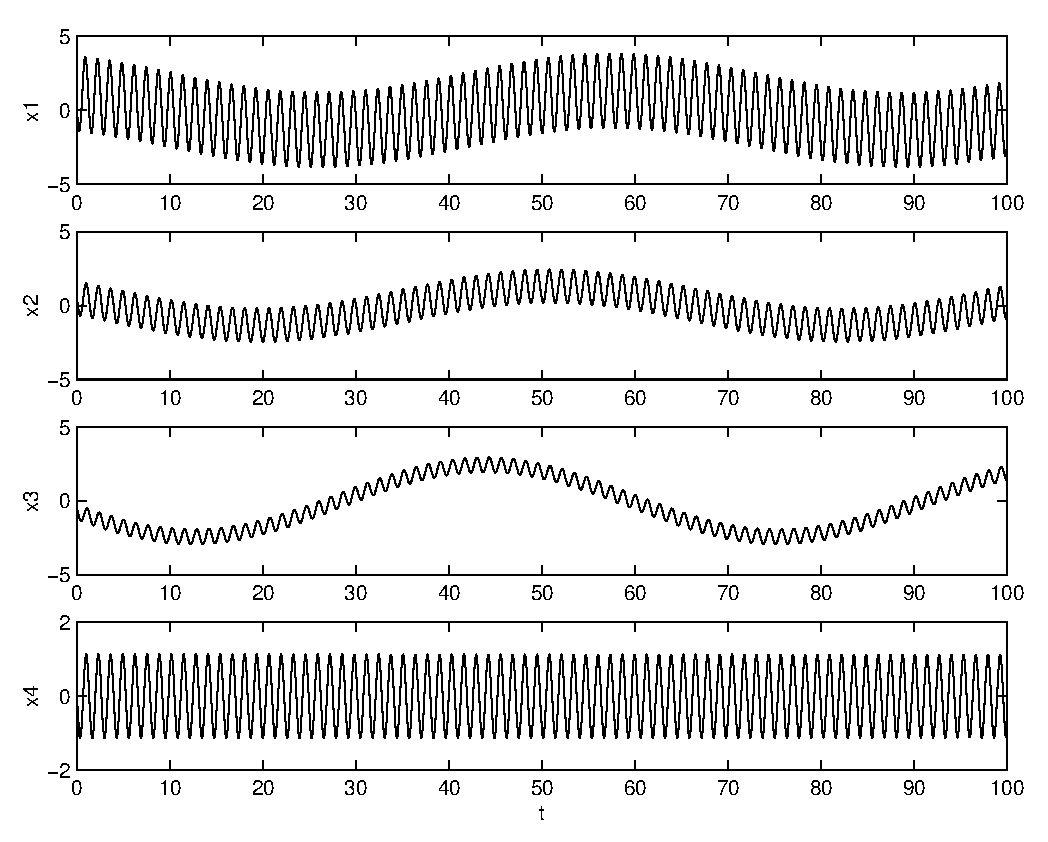
\psfig{file=../figures/ftor4ts.eps,width=5.3in}}
   \caption{Time series showing quasiperiodic two-frequency motion for the 
	solution of the linear system \protect\eqref{e:tor4} with initial 
	condition $X_0=(0.2,0.6,-0.5,0.1)$.}
   \label{F:ftor4ts}
\end{figure}

The phase space portrait can be viewed in three dimensions (by just 
ignoring one coordinate).  The projections of this trajectory onto the 
$x_1x_3x_4$ hyperplane and the $x_1x_2x_4$ hyperplanes are given in 
Figure~\ref{F:ftorphase}.  There we can see the torus\index{torus}.  For 
linear systems with two pairs of complex conjugate purely imaginary
eigenvalues, almost all solutions lie on tori.  To verify this statement, 
experiment with different initial conditions and see Exercise~\ref{EX:tor4}. 

\begin{figure}[htb]
   \centerline{%
   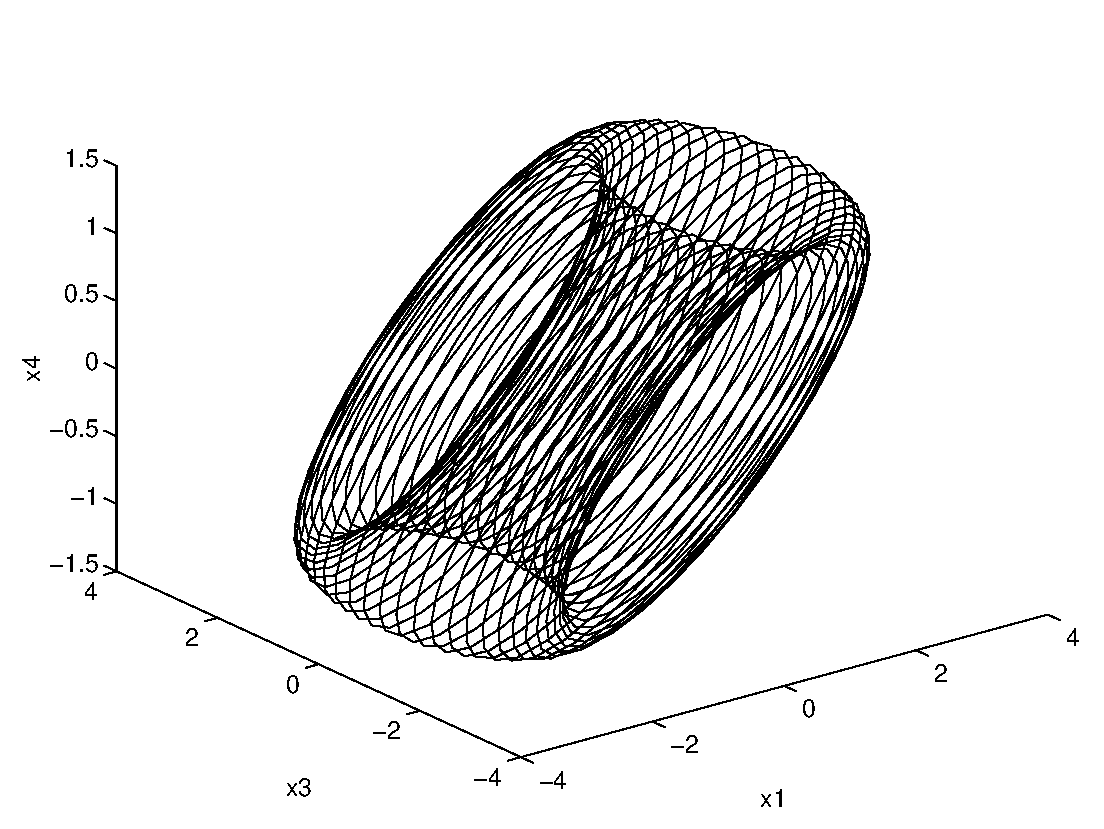
\psfig{file=../figures/ftor4ps1.eps,width=3.0in}
   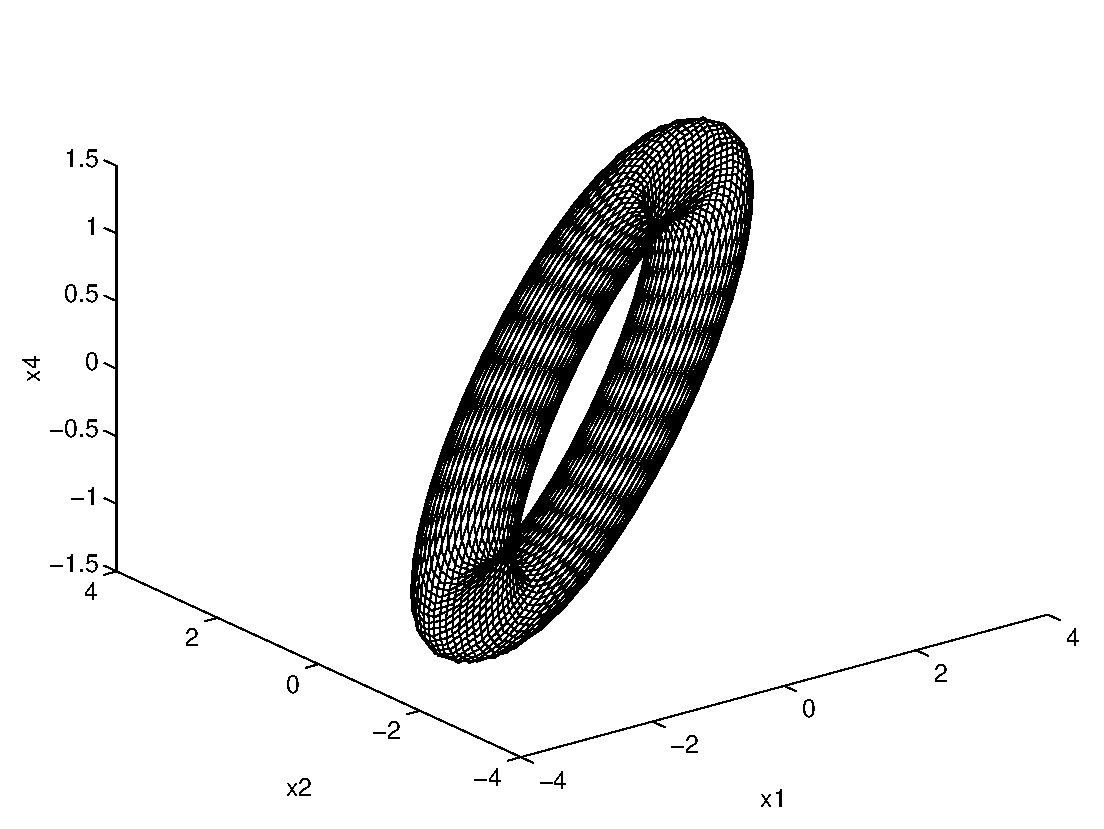
\psfig{file=../figures/ftor4ps2.eps,width=3.0in}}
   \caption{Phase space projections showing quasiperiodic motion on a torus of 
	the solution of the linear system \protect\eqref{e:tor4} with initial 
	condition $X_0=(0.2,0.6,-0.5,0.1)$.}
   \label{F:ftorphase}
\end{figure}

\subsection*{Asymptotically Stable Quasiperiodic Motion}
\index{motion!quasiperiodic}

In Section~\ref{S:HopfBif} we discussed Hopf bifurcation of planar autonomous 
systems that leads, by varying a parameter through a center, to an 
asymptotically stable periodic trajectory.  Here we discuss how we can also 
find asymptotically stable quasiperiodic motions\index{motion!quasiperiodic} 
in a similar way.  

\subsubsection*{Motion on a Torus in Four Dimensions}
\index{torus!in dimension four}

Consider the system of four differential equations 
\begin{matlabEquation}  \label{e:nonlintor}
\dot{X} = (A+\epsilon I_4)X - ||X||^2X,
\end{matlabEquation}
where $A$ has two pairs of complex conjugate purely imaginary eigenvalues
and $\epsilon>0$.  We see that $X=0$ is an equilibrium for \eqref{e:nonlintor}
and the Jacobian\index{matrix!Jacobian} 
matrix is $A+\epsilon I_4$ whose eigenvalues 
are $\lambda+\epsilon$ where $\lambda$ is an eigenvalue of $A$.  Since all 
of the eigenvalues of the Jacobian have positive real part, the origin is a 
source\index{source} in four dimensions.  On the other hand, the term 
$-||X||^2X$ in \eqref{e:nonlintor} always drives solutions toward the origin. 
The two forces balance and result in one asymptotically stable invariant 
torus.   The reasoning here is similar to that used to find limit cycles in
planar phase/amplitude equations.

Let $A$ be the matrix \eqref{e:tor4} and solve numerically the corresponding
differential equation \eqref{e:nonlintor} using the preloaded m-file 
{\tt f14\_5\_2.m}. That m-file is:
\begin{verbatim}
function f = f14_5_2(t,x)
A = [ 10.6722 -16.0417   5.4028 -12.2597;
       5.3472  -8.1375   2.7569  -3.6597;
       2.1574  -3.5194   1.1954  -0.3144;
       5.3287  -7.9931   2.6644  -3.7301];
f = (A+0.1*eye(4))*x - norm(x)^2*x;
\end{verbatim}\index{\computer!norm}
To solve this differential equation with initial conditions 
$X_0=(0.2,0.6,-0.5,0.1)$, type
\begin{verbatim}
[t,x] = ode45('f14_5_2',[0 100],[0.2,0.6,-0.5,0.1]');
\end{verbatim}\index{\computer!ode45}

The time series for this nonlinear system are given in Figure~\ref{F:tornlts}.
Note the initial transient that is present before the solution settles 
down to a quasiperiodic motion\index{motion!quasiperiodic} on a torus.
\index{torus}  The phase space picture in the $x_1x_3x_4$ hyperplane is given 
in Figure~\ref{F:tornlps}.  Here the transient is more visible.
 
\begin{figure}[htb]
   \centerline{%
   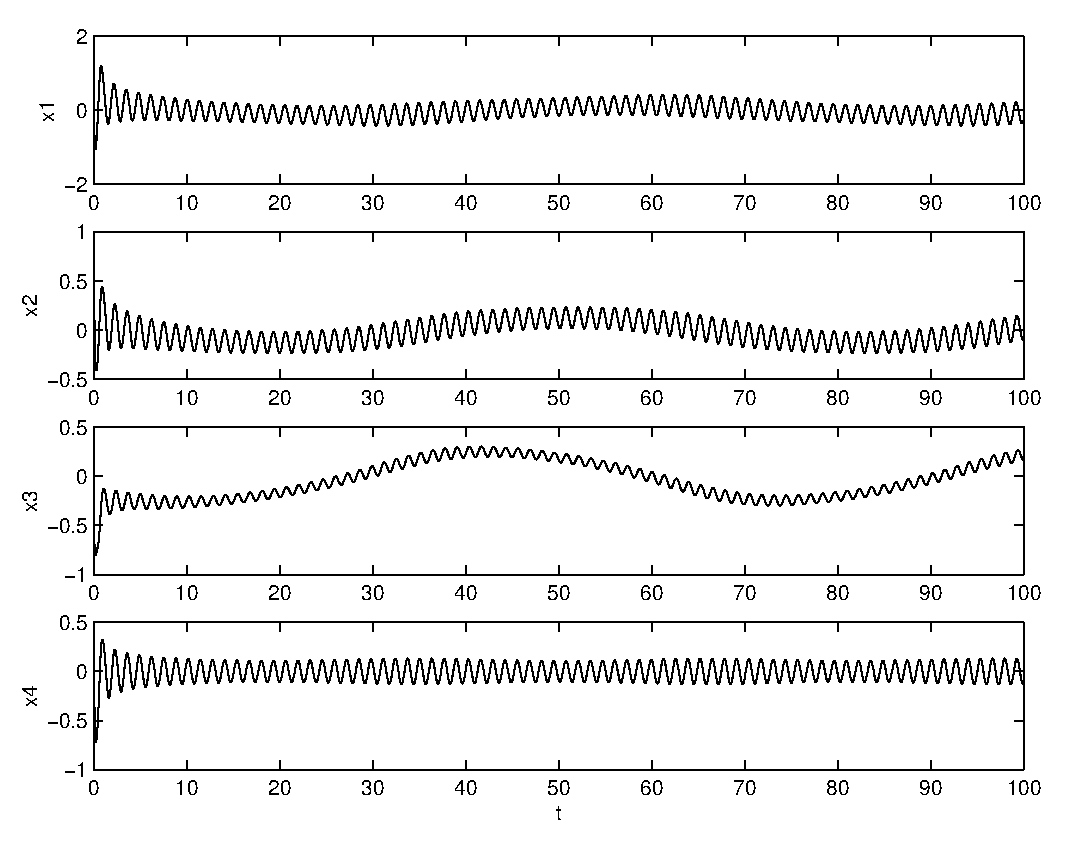
\psfig{file=../figures/ftornlts.eps,width=5.3in}}
   \caption{Time series showing quasiperiodic two-frequency motion for the 
	solution of the nonlinear system \protect\eqref{e:nonlintor} with 
	initial condition $X_0=(0.2,0.6,-0.5,0.1)$.}
   \label{F:tornlts}
\end{figure}

\begin{figure}[htb]
   \centerline{%
   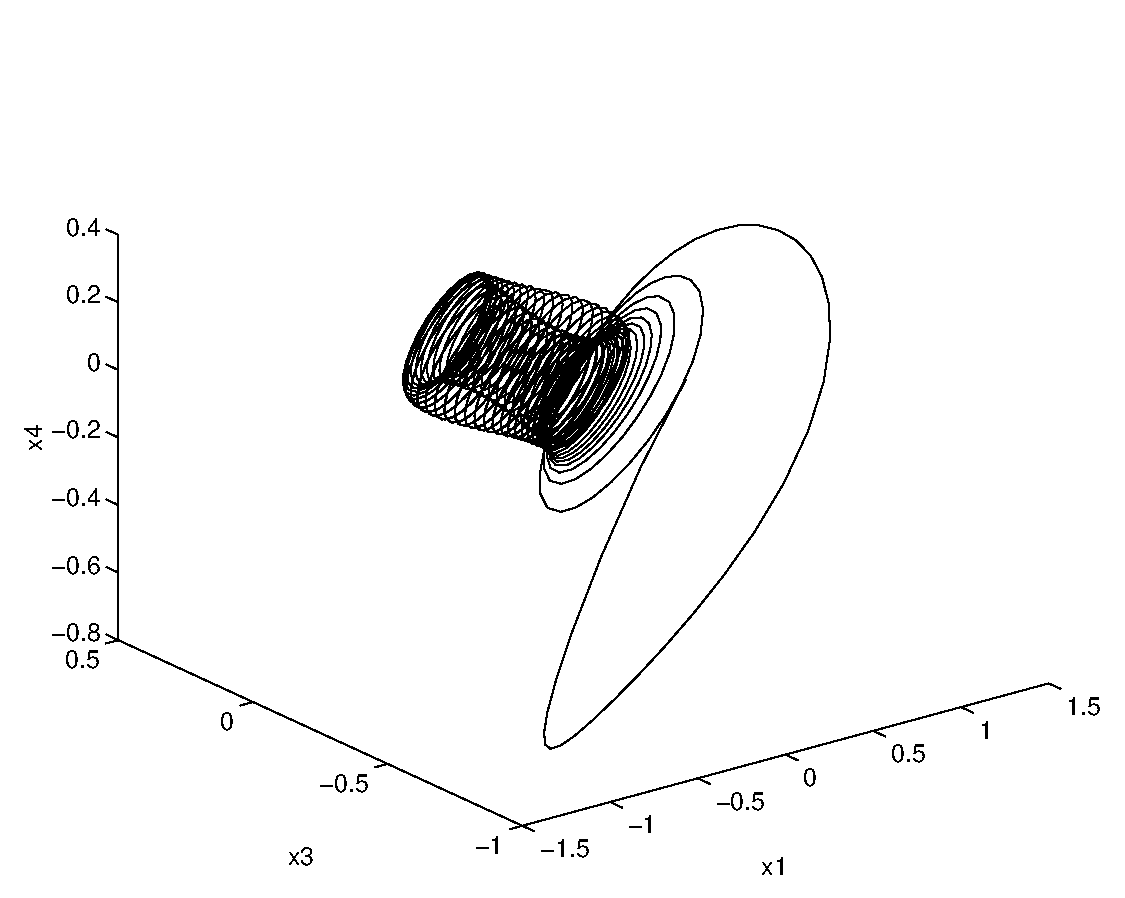
\psfig{file=../figures/ftornlps.eps,width=5.0in}}
   \caption{Phase space projections showing motion on a torus for the 
	solution of the nonlinear system \protect\eqref{e:nonlintor} with 
	initial condition $X_0=(0.2,0.6,-0.5,0.1)$.}
   \label{F:tornlps}
\end{figure}



\subsubsection*{A Torus in Three Dimensions}
\index{torus!in dimension three}

Until now, the way that we have constructed two frequency quasiperiodic 
solutions to systems of ODEs is based on having two independent frequencies 
present in a linear system.  It is not obvious --- yet it is true --- 
that solutions to nonlinear systems of three differential equations 
can also have two frequency quasiperiodic 
solutions\index{motion!two frequency}.  The theory that 
leads to this example is beyond the scope of this book; nevertheless, we
now have the numerical techniques to see (visually) that such solutions 
exist.

Consider the autonomous nonlinear system of ODEs\footnote{This system of
equations is taken from W.F. Langford, Numerical studies of torus bifurcations, 
ISNM {\bf 70}, Birkh\"auser, 1984.}:
\begin{matlabEquation}  \label{e:ftor3}
\begin{array}{rcl}
\dot{x}_1 & = & (x_3-0.7)x_1 - 3.5x_2\\
\dot{x}_2 & = &  3.5x_1 + (x_3-0.7)x_2 \\
\dot{x}_3 & = & 0.6 + x_3 - 0.33x_3^3 - (x_1^2+x_2^2)(1+.25x_3).
\end{array}
\end{matlabEquation}
The m-file for this system of equations is 
{\tt f14\_5\_3.m} and contains
\begin{verbatim}
function f = f14_5_3(t,x)
f = [(x(3)-0.7)*x(1) - 3.5*x(2); 
     3.5*x(1) + (x(3)-0.7)*x(2); 
     0.6 + x(3) - x(3)^3/3 - (x(1)^2+x(2)^2)*(1+0.25*x(3))];
\end{verbatim}
The differential equation \eqref{e:ftor3} is solved by typing
\begin{verbatim}
[t,x] = ode45('f14_5_3',[0 100],[0.1,0.03,0.001]');
\end{verbatim}\index{\computer!ode45}
The time series for the system \eqref{e:ftor3} are given in 
Figure~\ref{F:tor3ts} and the three dimensional phase space
\index{phase!space} picture is given in Figure~\ref{F:tor3ps}.

\begin{figure}[htb]
   \centerline{%
   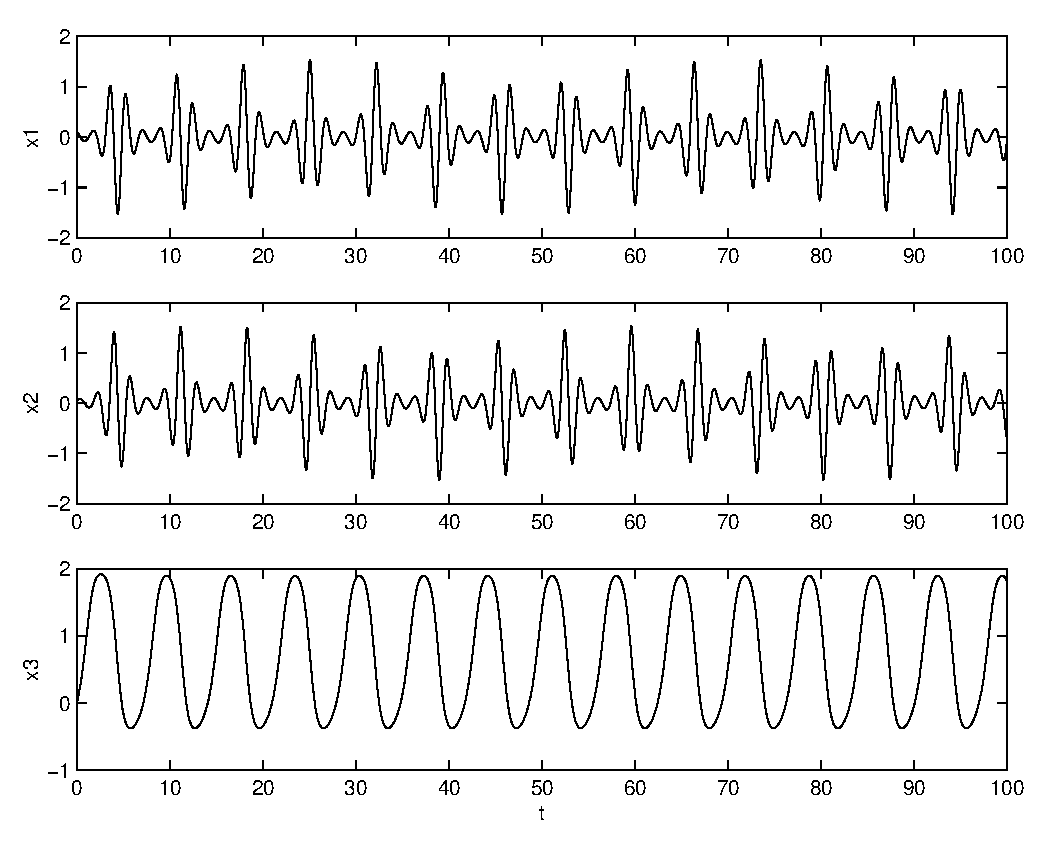
\psfig{file=../figures/ftor3ts.eps,width=5.0in}}
   \caption{Time series showing quasiperiodic two-frequency motion for the 
	solution of the nonlinear system \protect\eqref{e:ftor3} with initial 
	condition $X_0=(0.1,0.03,0.001)$.}
   \label{F:tor3ts}
\end{figure}

\begin{figure}[htb]
   \centerline{%
   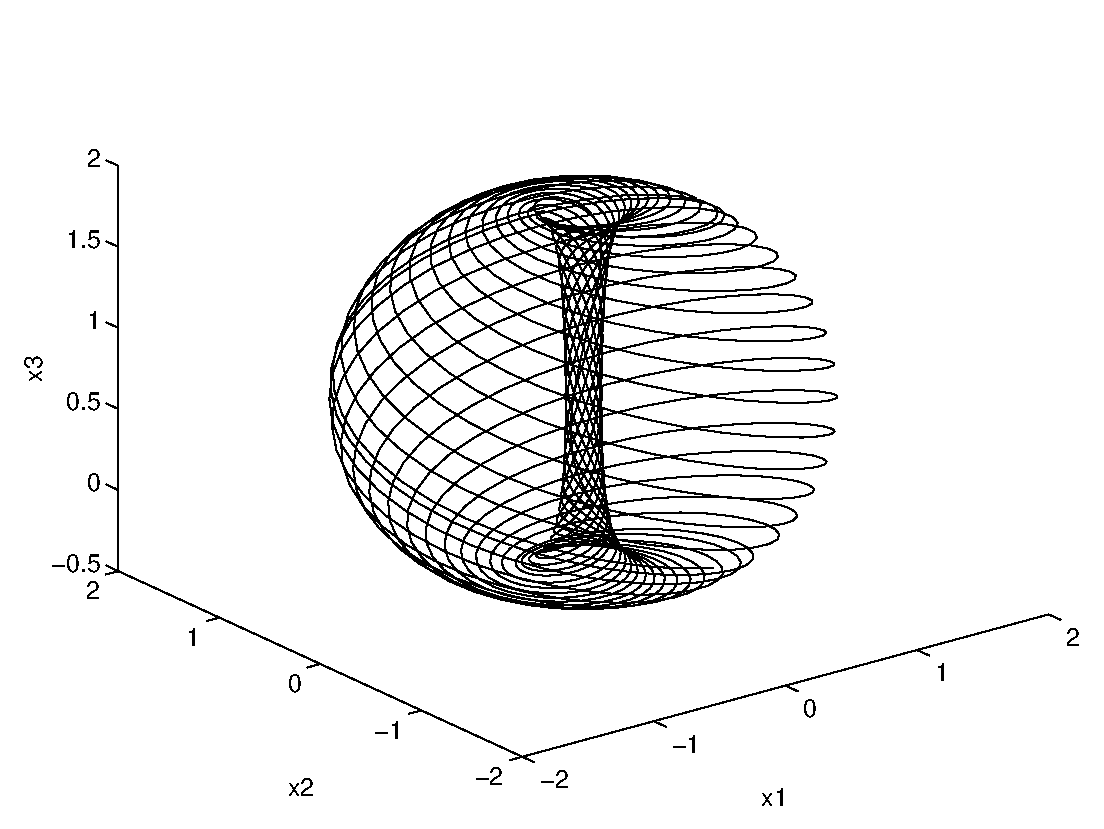
\psfig{file=../figures/ftor3ps.eps,width=5.0in}}
   \caption{Phase space showing motion on a torus for the solution trajectory 
	of the nonlinear system \protect\eqref{e:ftor3} with initial condition 
	$X_0=(0.1,0.03,0.001)$.}
   \label{F:tor3ps}
\end{figure}


\EXER

\CEXER

\begin{exercise}  \label{EX:tor4}
Let A be the $4\times 4$ torus example given in \eqref{e:tor4}.  Choose three 
different initial conditions to the system of ODEs $\dot{X}=AX$ and use 
{\tt ode45} compute solutions with these initial conditions.  (To decrease 
the length of time needed by the computer to do these calculations, shorten 
the time period to say $[0,30]$.)  
\begin{itemize}
\item[(a)]  Based on these calculations, verify that most initial conditions 
lead to quasiperiodic toroidal motions.  Display both time series and 
three dimensional phase portraits of your solutions. 
\item[(b)]  Take as initial condition the real part of one of the complex
eigenvectors of $A$.  (You will need to use \Matlab to find the eigenvalues
and eigenvectors of $A$.)  What kind of phase space motion do you see now? 
How does this solution differ from the toroidal motions obtained in (a)? 
Use Jordan normal forms to explain why your numerical answer is correct.
\end{itemize}
\end{exercise} 

\noindent In Exercises~\ref{c14.5.2a} -- \ref{c14.5.2d} use \Matlab to find
out whether the system of differential equations $\dot X= AX$ for
the given matrix $A$ has quasiperiodic solutions.
\begin{exercise} \label{c14.5.2a}
\begin{matlabEquation}\label{MATLAB:57}
A=\left(\begin{array}{rrrr}
    4.9666  &  2.2833  &  0.8000  &  5.3666\\
   -0.9889  & -0.0944  & -1.6000  & -1.7889\\
    2.9889  &  4.0944  & -0.4000  &  1.7889\\
   -8.9443  & -4.4721  &       0  & -4.4721
\end{array}\right).
\end{matlabEquation}
\end{exercise}

\begin{exercise} \label{c14.5.2b}
\begin{matlabEquation}\label{MATLAB:58}
A=\left(\begin{array}{rrrr}
    2.7666  &  0.2833  &  1.4000  &  4.5666\\
    2.4111  &  1.9056  & -1.8000  & -0.1889\\
   -0.4111  &  2.0944  & -0.2000  &  0.1889\\
   -7.9443  & -2.4721  & -1.0000  & -4.4721
\end{array}\right).
\end{matlabEquation}
\end{exercise}

\begin{exercise} \label{c14.5.2c}
\begin{matlabEquation}\label{MATLAB:59}
A=\left(\begin{array}{rrrrr}
    0.7130  & 24.8184  & 32.0740  &  2.8959  & 15.3610\\
    0.0552  & 17.0732  & 21.1395  &  6.6120  & 11.0843\\
   -0.6168  &-12.0764  &-16.0165  & -1.6151  & -7.3997\\
    1.0410  & -3.3312  & -2.0820  & -3.3312  & -3.1230\\
   -0.5205  &  1.6656  &  1.0410  &  1.6656  &  1.5615
\end{array}\right).
\end{matlabEquation}
\end{exercise}

\begin{exercise} \label{c14.5.2d}
\begin{matlabEquation}\label{MATLAB:60}
A=\left(\begin{array}{rrrrr}
  -10.2870 &  40.8184 &  30.0740 &  19.8959 &  38.3610\\
   -7.4448 &  25.0732 &  16.1395 &  15.8620 &  26.0843\\
    6.8833 & -20.0764 & -11.0165 & -10.3652 & -21.3998\\
    1.0410 &  -3.3312 &  -2.0820 &  -3.3312 &  -3.1230\\
   -0.5205 &   1.6656 &   1.0410 &   1.1656 &   0.5615
\end{array}\right).
\end{matlabEquation}
\end{exercise}


\end{document}
